\documentclass{beamer}
\usepackage{amsmath,amssymb}
\usepackage{graphicx}
%\usepackage{enumitem}
\usepackage{setspace}
\doublespacing
\usepackage{subcaption}
\usepackage[backend=biber]{biblatex}
\addbibresource{references.bib}
\usepackage{tikz}
\usepackage{pgfplots}
\pgfplotsset{compat=1.18}
\setbeamertemplate{caption}[numbered]
\renewcommand{\figurename}{Fig.}

\usetheme{madrid}


\title[PCA]{Principal Component Analysis}
\subtitle{Origins and Theories}
\author{Pooria Assarehha \vspace{-3mm}}
\institute{Department of Mathematics, Statistics \\ and Computer Science}
\date{\empty}

\AtBeginSection[]{
  \begin{frame}{Outline}
    \tableofcontents[currentsection]
  \end{frame}
}


\begin{document}
\graphicspath{{./figs/}}

\begin{frame}
    \titlepage
    \vspace{-1.5cm}
    \begin{center}
        \includegraphics[width=0.2\textwidth]{ut.png}
    \end{center}
    \vspace{-5mm}
    \centering \small Spring 2025
\end{frame}

\section{History}
\begin{frame}{History of PCA}
    \begin{figure}
        \begin{subfigure}[t]{0.35\textwidth}
            \includegraphics[width=\textwidth]{Karl_Pearson,_1910_(cropped).jpg}
            \caption{Pearson, Karl (1857 - 1936) in London 1910}
        \end{subfigure}
        \hfill
        \begin{subfigure}[t]{0.55\textwidth}
            \includegraphics[width=\textwidth]{Hotelling_1946.png}
            \caption{Hotelling, Harold (1895 - 1973) North Carolina 1946}
        \end{subfigure}
    \end{figure}
    \vspace{-3mm}
    \begin{itemize}
        \item Principal Axis Theorem in mechanics and geomery
        \item Karl Pearson, 1901 \cite{pearson1901}
        \item Harold Hotelling, 1933 \cite{hotelling1933}
    \end{itemize}
\end{frame}


\begin{frame}{Principal Axis Theorem}
    \begin{itemize}
        \item Principal Axis are perpendicular
        \begin{figure}
            \begin{subfigure}{0.4\textwidth}
                \includegraphics[width=\textwidth]{Ellipsoide.png}
                \subcaption{Ellipsode, Wikipedia}
            \end{subfigure}\hfill
            \begin{subfigure}{0.4\textwidth}
                \includegraphics[width=\textwidth]{Hyperboloid1.png}
                \subcaption{Hyperboloid, Wikipedia}
            \end{subfigure}
        \end{figure}
        \item represented as Quadratic forms \(f(x) = x^TAx = 0\)
    \end{itemize}
\end{frame}

\begin{frame}{In Linear Algebra}
    \begin{itemize}
        \item \textbf{Theorem:} \(A\) symmetric then exist Orthogonal \(Q\) such
        \[ A = Q \Lambda Q^T \qquad \text{(Spectral decomposition)}\]
        \item rows of \(Q\) eigenvectors of \(A\) and \(
            \Lambda = \begin{bmatrix}
                \lambda_1 & 0 &\dots  \\
                0 & \lambda_2 & \dots \\
                \vdots & \vdots & \ddots \\
            \end{bmatrix} \)
        \begin{eqnarray*}
            f(x) = x^TAx &=& x^TQ \Lambda Q^Tx  \\
            &\Rightarrow & z = Q^Tx \ , \quad  f(z) = z^T\Lambda z = 0
        \end{eqnarray*}
        \item \(z\) is a rotated Axis, \textcolor{red}{Notice!}
    \end{itemize}
\end{frame}


\begin{frame}{Karl Pearson (1901)}
    \begin{columns}
        \column{0.6\textwidth}
        \begin{itemize}
        \item Find the line/plane of closest fit
        \item Geometric view
        \item Minimize mean square perpendicular distance:
        \[
            \min_{\mathbf{w}} \sum_{i=1}^n \| \mathbf{x}_i - (\mathbf{x}_i \cdot \mathbf{w})\mathbf{w} \|^2
        \]
        \item Unsupervised fitting
    \end{itemize}
    \column{0.39\textwidth}
    \begin{figure}
        \includegraphics[width=\textwidth]{PCA3d.png}
        \caption{From ESL, Tibshirani, Hastie}
    \end{figure}
    \end{columns}
    
\end{frame}


\begin{frame}{Harold Hotelling (1933)}
    \begin{itemize}
        \item Statistical view
        \item Find directions of maximum variance:
        \[
            \max_{\|\mathbf{v}\| = 1} \text{Var}(\mathbf{v_i}^TX) 
        \]
        \item \(X \ \sim \ N_p(\mu, \Sigma)\)
        \item Derived with Lagrange, No mention of \(\hat{\Sigma}\)
    \end{itemize}
\end{frame}

\section{Derivation}


\begin{frame}{Maximization Lemma}
    \begin{itemize}
        \item \textbf{Maximization Lemma:} For symmetric $\Sigma$, \[ \max_{\|\mathbf{v}\| = 1} \mathbf{v}^T \Sigma \mathbf{v} = \max_i \lambda_i\]
        \item \textbf{Goal of Hotelling:} find direction $\mathbf{v}$ s.t. variance of projection is maximized
        \[
            \max_{\|\mathbf{v}\| = 1} \text{Var}(\mathbf{v}X) = \mathbf{v}^T \text{Var}(X)\mathbf{v} = \mathbf{v}^T \Sigma \mathbf{v}
        \]
        \item \(v_{\max}\) is the eigenvector of \(\lambda_{\max}\)
    \end{itemize}
\end{frame}

\begin{frame}{The Transformation} 
\begin{itemize}
    % \item if columns \(X\) are centered (Later on) then \(\Sigma = X^TX\) 
    \item Symmetric of cource hence \(\Sigma = Q\Lambda Q^T\)
    \item rows of \(Q, \Lambda\) can be permuted such
    \begin{eqnarray*}
        \Lambda = \begin{bmatrix}
            \lambda_1 & 0 &\dots  \\
            0 & \lambda_2 & \dots \\
            \vdots & \vdots & \ddots \\
        \end{bmatrix} \quad \lambda_1 \ge \lambda_2 \ge\dots \lambda_d \le 0
    \end{eqnarray*}
    \item \(Z_{n\times p} = XQ^T \) columns Ordered in Variance \textcolor{red}{No Correlation!}
\end{itemize}
\end{frame}


\section{Results}
\begin{frame}{Dimention Reduction}
    \begin{itemize}
        \item \(\Sigma\) \textbf{not} always \textbf{full-rank}, \(\exists q \ s.t. \ q <  i \le p \ \lambda_i = 0\)
        \item Then \(Z = XQ^T\) has ending columns of Zero!
        \item Good For Us! Let \(Q_q\) first \(q\) rows of \(Q\) hence \(q\times p\)
        \item \(Z_q = XQ_q^T\) is now \(n\times q\) (reduced dimentions) 
        \item And Without loss of info, Let's create a metric.
    \end{itemize}
\end{frame}

\begin{frame}{Variance Explained}
    \begin{itemize}
        \item Choosing \(q\) How much of Variance saved?
        \[h(q) = \frac{\sum_i^q \lambda_i}{\sum_i^p \lambda_i } \quad , \quad q = 1, \dots , p \] 
        \item \( 0 \le h(q) \le 1 \) increasing
        \item final \(\lambda_i\) might be very small
        \item \(Z_q = XQ^T_q\) much smaller dimension, most of variance
        \item \(\text{Var}(Z) = \text{Var}(XQ^T_q) = Q_q\text{Var}(X)Q^T_q = \Lambda_q\)
    \end{itemize}
\end{frame}

\begin{frame}{Scree Plot}
    \begin{center}
    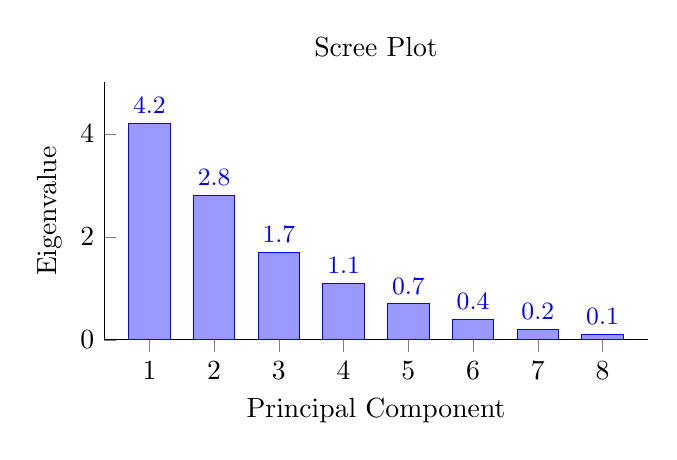
\begin{tikzpicture}
        \begin{axis}[
            width=0.7\textwidth,
            height=0.4\textwidth,
            ybar,
            bar width=15pt,
            ylabel={Eigenvalue},
            xlabel={Principal Component},
            symbolic x coords={1,2,3,4,5,6,7,8},
            xtick=data,
            ymin=0,
            ymax=5,
            nodes near coords,
            every node near coord/.append style={font=\small},
            axis y line*=left,
            axis x line*=bottom,
            enlarge x limits=0.1,
            title={Scree Plot}
        ]
        \addplot+[fill=blue!40] coordinates {
            (1,4.2) (2,2.8) (3,1.7) (4,1.1) (5,0.7) (6,0.4) (7,0.2) (8,0.1)
        };
        \end{axis}
    \end{tikzpicture}
    \end{center}
\end{frame}

\begin{frame}{PCA Geometric Interpretation}
    \begin{figure}
        \includegraphics[width=\textwidth]{PCA3d2d.png}
        \caption{Choose \(Z_2 = X Q_2\) and dimension is reduced}
    \end{figure}
\end{frame}

\section{Notices}
\begin{frame}{Centering And Scaling}
    \begin{itemize}
        \item Hotelling centered and scaled \(X\) (Why?)
        \item \(\bar{X}_{p\times 1} = 0\) and \(x_i^Tx = 1\) for each column.
        \item Centering allows \(\Sigma = X^TX\)
        \item Not scaling causes inflamation of \(\lambda_i\)
    \end{itemize}
\end{frame}

\begin{frame}{Linearity}
    \begin{itemize}
        \item The transformation is only linear
        \item \(Z_i\) are uncorrelated, Not independent
        \item Non-linear dependendece limits efficiency
    \end{itemize}
\end{frame}

\section{Applications}
\begin{frame}{PCA in Image Processing (Compression)}
    \begin{columns}
        \column{0.5\textwidth}
        \begin{itemize}
            \item Flatten: 2D to 1D
            \item \(Z_k = XQ_k^T\)
            \item Only top $k$ components
            \item \(X' = Z_k Q_k \) reconstruction of \(X\)
        \end{itemize}
        \column{0.5\textwidth}
        \includegraphics[width=\textwidth]{pca_5.png}
        \captionof{figure}{PCA-based image compression: original vs reconstruction}
    \end{columns}
\end{frame}

\begin{frame}{PCR: Principal Component Regression}
    \begin{itemize}
        \item LS fit on \(Z_k\) instead of whole \(X\) \cite{hastie2009}
        \item simmilar effect as penalization
        \item Good with Linearity assumption
    \end{itemize}
\end{frame}

\section{Extensions}
\begin{frame}{Principal Curves and Surfaces}
    \begin{itemize}
        \item Thesis by Hastie, 1989 \cite{Hastie01061989}
        \item Non-linear patternes in Data
    \end{itemize}
    \begin{figure}
        \includegraphics[width = \textwidth]{PCAsurface.png}
    \end{figure}
\end{frame}


\begin{frame}{Karhunen--Lo\`eve Theorem}
    \begin{itemize}
        \item $K(s,t) = \mathbb{E}[X(s)X(t)]$ — covariance function of process $X(t)$
        \item $X(t) = \sum_{i=1}^{\infty} Z_i \phi_i(t)$
        \begin{description}
            \item[$Z_i$] uncorrelated random variables (scores)
            \item[$\phi_i(t)$] orthonormal eigenfunctions of $K(s,t)$
        \end{description}
        \item Used in functional data analysis and signal processing
    \end{itemize}
\end{frame}

\begin{frame}{Alternatives}
    \begin{enumerate}
        \item  t-SNE: T-distributed Stochastic Neighbor Embeding \cite{JMLR:v9:vandermaaten08a}
    \begin{itemize}
        \item Emphasizes on local patterns
        \item Non-Linear suitable 
        \item Visualising Advantege
    \end{itemize}
    \item UMAP: Uniform Manifold Approximation and Projection \cite{McInnes_Healy_Melville_2018}
    \begin{itemize}
        \item From Riemannian geometry and algebraic topology
        \item Better computational complexity than t-SNE
        \item Preserves both local and global structure
    \end{itemize}
    \end{enumerate}

\end{frame}

% \section{Alternatives}

\section{References}
\begin{frame}[allowframebreaks]{References}
    \printbibliography
\end{frame}

\begin{frame}{For Your Attention}
    \centering
    \Large
    \emph{Thank You!}
\end{frame}

\end{document}
